% CVPR 2022 Paper Template
% based on the CVPR template provided by Ming-Ming Cheng (https://github.com/MCG-NKU/CVPR_Template)
% modified and extended by Stefan Roth (stefan.roth@NOSPAMtu-darmstadt.de)

\documentclass[10pt,onecolumn,letterpaper]{article}

%%%%%%%%% PAPER TYPE  - PLEASE UPDATE FOR FINAL VERSION
%\usepackage[review]{cvpr}      % To produce the REVIEW version
\usepackage{cvpr}              % To produce the CAMERA-READY version
%\usepackage[pagenumbers]{cvpr} % To force page numbers, e.g. for an arXiv version

% Include other packages here, before hyperref.
\usepackage{graphicx}
\usepackage{amsmath}
\usepackage{amssymb}
\usepackage{booktabs}


% It is strongly recommended to use hyperref, especially for the review version.
% hyperref with option pagebackref eases the reviewers' job.
% Please disable hyperref *only* if you encounter grave issues, e.g. with the
% file validation for the camera-ready version.
%
% If you comment hyperref and then uncomment it, you should delete
% ReviewTempalte.aux before re-running LaTeX.
% (Or just hit 'q' on the first LaTeX run, let it finish, and you
%  should be clear).
\usepackage[pagebackref,breaklinks,colorlinks]{hyperref}


% Support for easy cross-referencing
\usepackage[capitalize]{cleveref}
\crefname{section}{Sec.}{Secs.}
\Crefname{section}{Section}{Sections}
\Crefname{table}{Table}{Tables}
\crefname{table}{Tab.}{Tabs.}


%%%%%%%%% PAPER ID  - PLEASE UPDATE
\def\cvprPaperID{*****} % *** Enter the CVPR Paper ID here
\def\confName{CVPR}
\def\confYear{2022}


\begin{document}

%%%%%%%%% TITLE - PLEASE UPDATE
\title{Statistics Learning Project Report}

\author{Yilong Zhao\\
022033910058
%Institution1 address\\
}
% For a paper whose authors are all at the same institution,
% omit the following lines up until the closing ``}''.
% Additional authors and addresses can be added with ``\and'',
% just like the second author.
% To save space, use either the email address or home page, not both
%\and
%Second Author\\
%Institution2\\
%First line of institution2 address\\
%{\tt\small secondauthor@i2.org}
%}
\maketitle

%%%%%%%%% ABSTRACT
\begin{abstract}
   %The ABSTRACT is to be in fully justified italicized text, at the top of the left-hand column, below the author and affiliation information.
   %Use the word ``Abstract'' as the title, in 12-point Times, boldface type, centered relative to the column, initially capitalized.
   %The abstract is to be in 10-point, single-spaced type.
   %Leave two blank lines after the Abstract, then begin the main text.
   %Look at previous CVPR abstracts to get a feel for style and length.
   The task is to train a model on the training dataset and predict on a noised test set.
   I try two data processing methods, PCA and Reduced Rank LDA, to reduce the dimension of the samples.
   After that, I try three models, LDA, SVM, and MLP to fit the training dataset.
   K-fold cross-validation and AIC are used to evaluate the performance of the models.
   Results show that PCA is much better than Reduced Rank LDA on the noised test dataset.
   LDA can achieve the best test accuracy on the test dataset.
\end{abstract}

%%%%%%%%% BODY TEXT
\section{Data Processing}
\label{sec:data-processing}

\subsection{Principal Components Analysis (PCA)}
\label{sec:data-processing:pca}

The task is to train a model on the training dataset and predict on a noised test dataset.
The training set has 6666 pictures, while the test set have 2857 pictures.
Each picture has 1536 features.
This feature dimension is too large for models.
Therefore, I use principal components analysis (PCA) to reduce the dimension of features.
The steps of PCA are as follows:
\begin{enumerate}
    \item Substrate the mean value of each feature.
    \item Compute the covariance matrix with python function $np.cov$.
    \item Compute the covariance matrix's eigenvalue and eigenvector with python function $np.linalg.eig$, and sort the eigenvalue in descending order.
    \item Keep the first $N$ columns of eigenvectors, and use the $1536\times N$ submatrix to map the features from the original space to the new space.
\end{enumerate}

One key value to decide is the dimension of the new space $N$.
We use the following equation to compute the error of PCA:
\begin{equation}
    1 - \dfrac{\sum_{i=0}^N \lambda_i}{\sum_{i=0}^{1536} \lambda_i} < \varepsilon
    \label{eqn:pca-error}
\end{equation}
Where $\lambda_i$ is the $i^\mathrm{th}$ eigenvalue of the covariance matrix.
We set $\varepsilon=0.3$, and from \figurename{}~\ref{fig:pca}, the corresponding $N=112$.

\begin{figure}
    \centering
    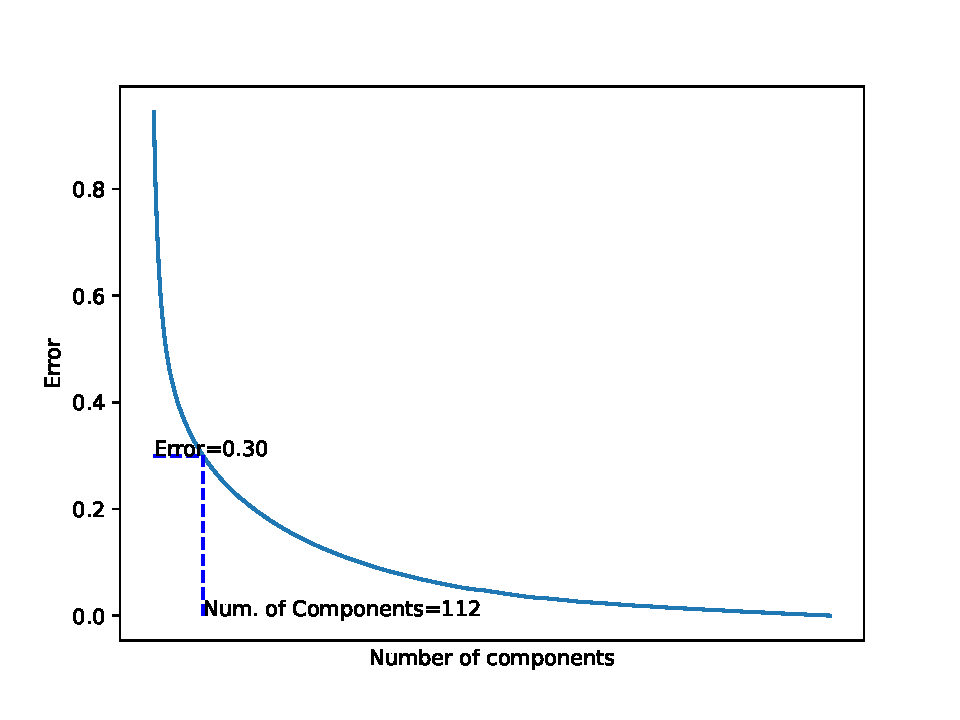
\includegraphics[width=0.9\linewidth]{figures/pca_components.pdf}
    \caption{Relationship between PCA error and the dimension of the new space $N$}
    \label{fig:pca}
\end{figure}


\subsection{Reduced Rank Linear Discriminant Analysis (Reduced Rank LDA)}
\label{sec:data-processing:rr-lda}

Another method to reduce the dimension is Reduced Rank Linear Discriminant Analysis (Reduced Rank LDA).
Unlike PCA, Reduced Rank LDA tries to find the discriminant direction which minimizes this overlap for Gaussian data.
The step is as follows:
\begin{enumerate}
    \item Estimate the centroid matrix $M_{k\times P}$, and the variance of the sample $W=\hat{\Sigma}$.
    \item Compute $M^*=MW^{-1/2}$.
    \item Compute $B^*$, the covariance matrix of $M^*$, and compute the eigenvector matrix $V^*$.
    \item The new discriminant variable is $Z_l=v_l^TX$, with $v_l=W^{-1/2}v_l^*$
\end{enumerate}

Note that the Reduced Rank LDA can only reduce the number of dimensions to $L-1$ dimensions, with $L=20$ being the number of classes.
Therefore, compared to PCA, Reduced Rank LDA loses too much information.
We will discuss this in the experiment Section \ref{sec:model-selection}.
\section{Linear Discriminant Analysis (LDA)}
\label{sec:lda}

The first classification model I try is Linear Discriminant Analysis (LDA).
This means that we introduce an assumption that the distribution is the same among different classes.
A linear line is used to distinguish between the classes.
The LDA Rule is:
\begin{eqnarray}
    \delta_k\left(x\right) & = & x^T\Sigma^{-1}\mu_k - \dfrac{1}{2}\mu_k\Sigma^-1\mu_k+\log\pi_k
    \label{eqn:lda-rule}
\end{eqnarray}
where $\mu_k$ is the mean of the $k^{\mathrm{th}}$ class, $\pi_k$ is the proportion of class $k$, $\Sigma$ is the variance of the samples.
For each category $k=1,...,20$, we compute the score $\delta_k(x)$.
The class of the sample is the category with the maximum $delta_k(x)$ value.

The parameters are estimated by:
\begin{eqnarray}
    \hat{\pi}_k & = & \dfrac{N_k}{N} \\
    \hat{\mu}_k & = & \sum_{g_i=k}x_i\/N_k \\
    \hat{\Sigma} & = & \sum_{k=1}^{K}\sum_{g_i=k} \left(x_i-\hat{\mu}_k\right)\left(x_i-\hat{\mu}_k\right)^T / \left(N-K\right)
\end{eqnarray}

\section{Support Vector Machine (SVM)}
\label{sec:svm}

The second classification model I try is the support vector machine (SVM).
SVM uses a linear surface to distinguish between two classes.
The aim of SVM is to maximize the distance between the linear surface and support vectors.
However, the problem is an ill-posed problem.
Therefore, instead of solving the original problem, I try to solve the dual problem.

The first step is to solve a quadratic programming (QP) problem:
\begin{eqnarray}
    \max_\alpha & \mathcal{L} = -\dfrac{1}{2}\sum_{i=1}^{n}\sum_{j=1}^{n}\alpha_i\alpha_jy_iy_jK\left(x_i, x_j\right) + \sum_{i=1}^{n}\alpha_i \\
    s.t. & \alpha_i \geqslant 0 \\
     & \sum_{i=1}^{n} \alpha_iy_i = 0
    \label{eqn:svm-qp}
\end{eqnarray}

We solve the QP problem with Python library \textit{cvxopt}.
We use the function \textit{cvxopt.solvers.qp(P,q,G,h,A,b)} to solve the QP problem:
\begin{eqnarray}
    \min & \dfrac{1}{2} x^TPx + q^T x \\
    s.t. & Gx \leqslant h \\
     & Ax = b
\end{eqnarray}
Therefore, the parameters are:
\begin{eqnarray}
    P & = & y y^T .* K(x,x) \\
    q & = & -1 \\
    G & = & - \mathcal{I} \\
    h & = & 0 \\
    A & = & y \\ 
    b & = & 0
\end{eqnarray}


Then we select the samples with $\alpha>0$ as support vector $x_{t_j}$.
However, none of the $\alpha$ in the solution is strictly 0 due to the computational error.
To address this, we manully set a threshold $\alpha_{tr}=1e-6$, and reguard $\alpha_i<\alpha_{tr}$ as 0.
Then a new sample $z$ can be classified with:
\begin{eqnarray}
    \hat{y} & = & \mathrm{sgn}\left(\alpha_t\cdot y_t\cdot \left(x_t^Tz\right)\right)
    \label{eqn:svm-pred}
\end{eqnarray}

For every two classes, we train an SVM model to classify them.
As there are 20 classes, we train 190 SVM models.
Given a test sample, each SVM model votes on it.
The class with the most votes is regarded as the result of the classification.

The kernel function $K\left(x_i, x_j\right)$ is decided using model selection.
We consider the polynomial kernel function:
\begin{eqnarray}
    K\left(x_i, x\right) & = & \left(x_i^T\cdot x +1\right)^p
    \label{eqn:svm-kernel}
\end{eqnarray}
In model selection, we test the order $p=1,2,3$ and select the best value of the order.
\section{Multilayer Perceptron (MLP)}
\label{sec:mlp}

The third model I try is Multilayer Perceptron (MLP).
I directly use the MLP model provided by \textit{sklearn} library.
The activation function is ReLU, and the optimizer is Adam.
We scan different hidden neuron number in the experiment Section \ref{sec:model-selection}.
\section{Model Selection}
\label{sec:model-selection}

\subsection{K-fold Cross Validation}
\label{sec:model-selection:k-fold}

I use K-fold cross-validation to perform model selection.
The training set is randomly divided into K sub-sets.
Given a model $f$, we train the model with removing $k^{\mathrm{th}}$ fold data, and use the $k^{\mathrm{th}}$ fold data to test the model:
\begin{eqnarray}
    CV\left(\hat{f}\right) & = & \dfrac{1}{N}\sum_{i=1}^{N} L\left(y_i,\hat{f}^-k\left(x_i\right)\right)
    \label{eqn:cv}
\end{eqnarray}

\subsection{Akaike information criterion (AIC)}
\label{sec:model-selection:aic}

The second model selection method is the Akaike information criterion (AIC).
The AIC equation is:
\begin{eqnarray}
    AIC\left(\alpha\right) & = & \overline{err}\left(\alpha\right) + 2 \dfrac{d\left(\alpha\right)}{N}
    \hat{\sigma}_\varepsilon^2
\end{eqnarray}
where $\overline{err}\left(\alpha\right)$ is the training error, and $d\left(\alpha\right)$ is the number of parameters.

\subsection{Results}
\label{sec:model-selection:results}
\begin{table}
    \centering
    \caption{Models}
    \label{tab:models}
    \begin{tabular}{c|c}
        \hline\hline
        Model & Description \\\hline\hline
        Reduced Rank LDA & LDA model; Reduce dimension with Reduced Rank LDA ($N=19$) \\
        PCA + LDA & LDA model; Reduce dimension with PCA ($N=112$) \\
        PCA + SVM-1 & SVM model with linear kernel; Reduce dimension with PCA ($N=112$) \\
        PCA + SVM-2 & SVM model with kernel $p=2$; Reduce dimension with PCA ($N=112$) \\
        PCA + SVM-3 & SVM model with kernel $p=3$; Reduce dimension with PCA ($N=112$) \\
        PCA + MLP-100 & MLP model with 100 hidden neurons; Reduce dimension with PCA ($N=112$) \\
        PCA + MLP-200 & MLP model with 200 hidden neurons; Reduce dimension with PCA ($N=112$) \\
        PCA + MLP-300 & MLP model with 300 hidden neurons; Reduce dimension with PCA ($N=112$) \\
        PCA + MLP-400 & MLP model with 400 hidden neurons; Reduce dimension with PCA ($N=112$) \\
        \hline
    \end{tabular}
\end{table}

The models we compare are listed in \tablename{}~\ref{tab:models}.
We compare LDA, three SVM models with different kernels, and 4 MLP models with different hidden neuron numbers.
The cross-validation is listed in \tablename{}~\ref{tab:cv-result}.
The best model is MLP with 400 hidden neurons.
Both LDA and MLP can achieve relatively high accuracy.

Then we compare the two data processing methods, PCA and Reduced Rank LDA.
We add noise under standard normal distribution to the validation set.
\figurename{}~\ref{fig:rrlda_lda_cv_noise} and \figurename{}~\ref{fig:pca_lda_cv_noise} depicts the relation between cross-validation and noise of reduced rank LDA and PCA.
Reduced rank LDA can barely tolerate noise.
Even a slight noise with a variance of 0.0001 can severely affect the predict accuracy.
While for PCA, the noise does not influence the accuracy much.

\begin{figure}
    \centering
    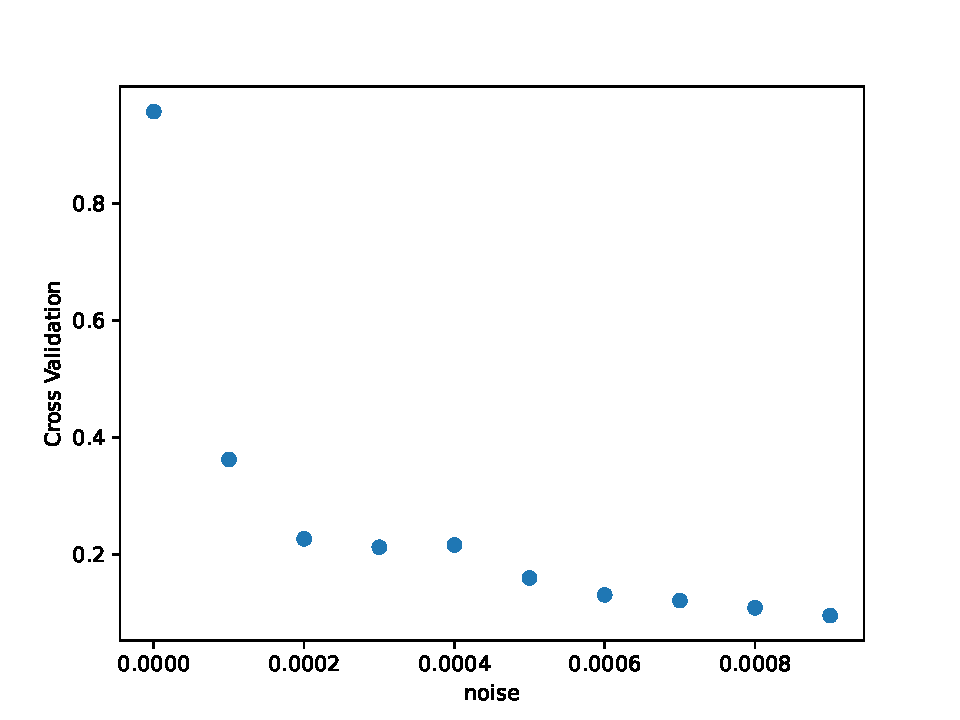
\includegraphics[width=0.7\linewidth]{figures/rrlda_lda_cv_noise.pdf}
    \caption{Cross validation of Reduced Rank LDA under different noise variance.}
    \label{fig:rrlda_lda_cv_noise}
\end{figure}

\begin{figure}
    \centering
    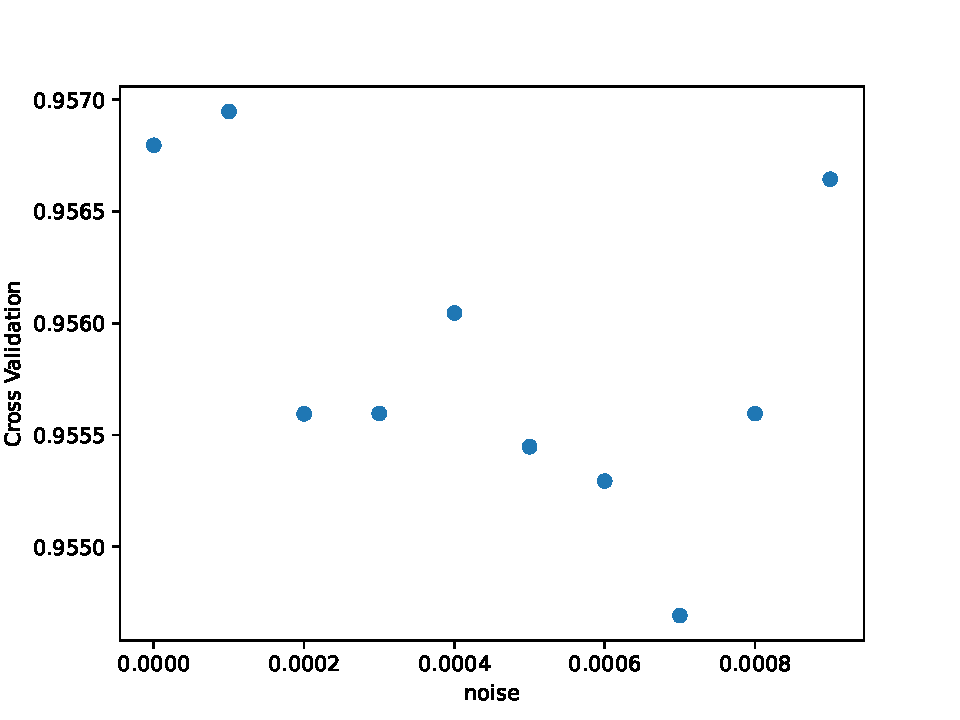
\includegraphics[width=0.7\linewidth]{figures/pca_lda_cv_noise.pdf}
    \caption{Cross validation of PCA under different noise variance.}
    \label{fig:pca_lda_cv_noise}
\end{figure}

\begin{table}
    \centering
    \caption[short]{Cross Validation and AIC Result}
    \label{tab:cv-result}
    \begin{tabular}{c|ccc}
        \hline\hline
        Model & AIC & CV & Accuracy\\ \hline\hline
        Reduced Rank LDA &  & 0.9541 & 0.0560 \\
        PCA + LDA & 0.9649 & 0.9548 & 0.9447 \\
        PCA + SVM-1 & 0.7858 & 0.7790 & 0.7647 \\
        PCA + SVM-2 & 0.0489 & 0.0489 & 0.0378 \\
        PCA + SVM-3 & 0.0489 & 0.0489 & 0.0378 \\
        PCA + MLP-100 & 1.0 & 0.9532 & 0.9251 \\
        PCA + MLP-200 & 1.0 & 0.9551 & 0.9286 \\
        PCA + MLP-300 & 1.0 & 0.9535 & 0.9321 \\
        PCA + MLP-400 & 1.0 & 0.9577 & 0.9349 \\
        \hline\hline
    \end{tabular}
\end{table}
\section{Accuracy}
\label{sec:accuracy}

We test the models in \tablename{}~\ref{tab:models} on the test set, and get the accuracy from the Kaggle platform.
Results are listed in \figurename{}~\ref{fig:result-kaggle} and \figurename{}~\ref{fig:result-rrlda}.
The LDA model can achieve the best accuracy 94.47\%.
For reduced rank LDA, the test accuracy is much lower than the cross-validation accuracy.
This is because the test set samples are noised, and reduced rank LDA cannot tolerate noise.

\begin{figure}
    \centering
    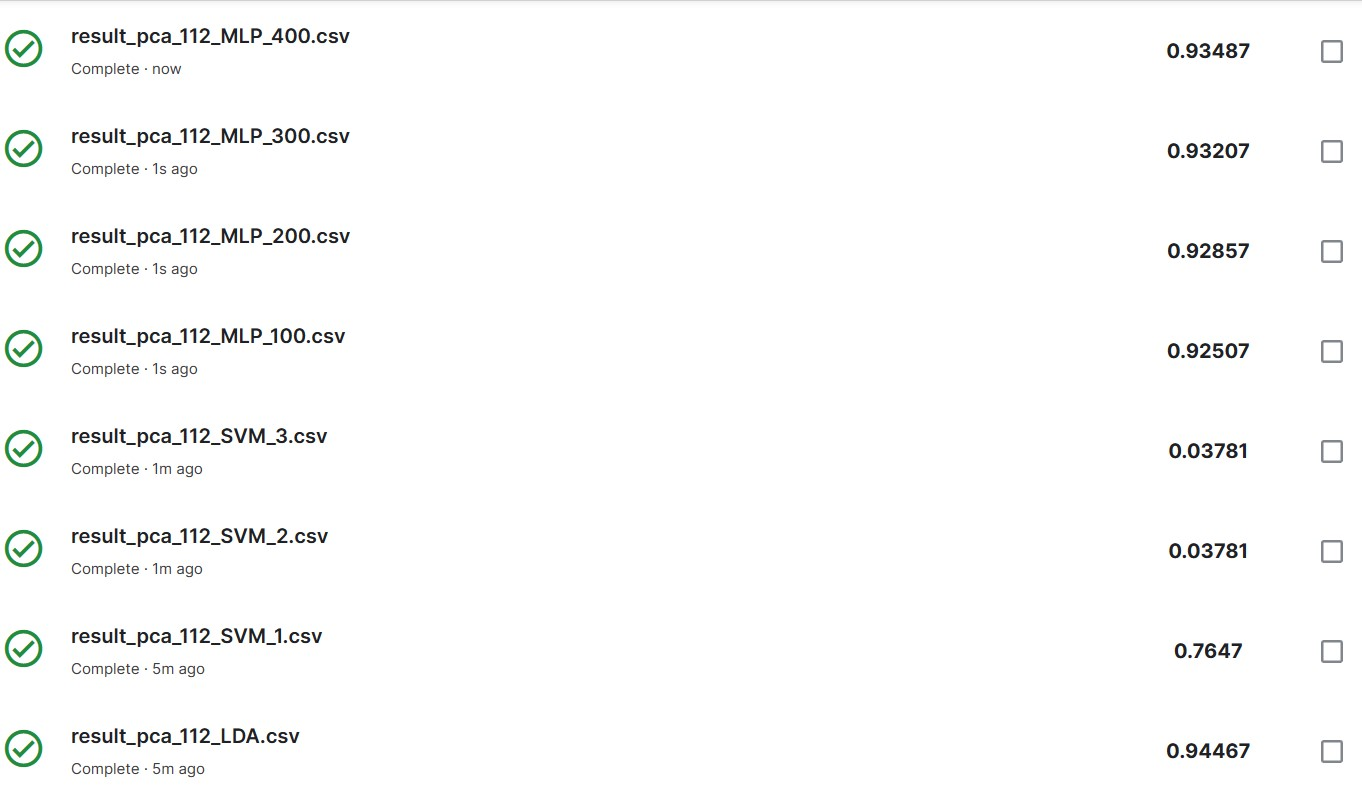
\includegraphics[width=\linewidth]{figures/kaggle.jpg}
    \caption{Accuracy result from Kaggle.}
    \label{fig:result-kaggle}
\end{figure}


\begin{figure}
    \centering
    
\includegraphics[width=\linewidth]{figures/rr-lda.jpg}
    \caption{Accuracy result of Reduced Rank LDA from Kaggle.}
    \label{fig:result-rrlda}
\end{figure}
%\section{Introduction}
%\label{sec:intro}
%
%Please follow the steps outlined below when submitting your manuscript to the IEEE Computer Society Press.
%This style guide now has several important modifications (for example, you are no longer warned against the use of sticky tape to attach your artwork to the paper), so all authors should read this new version.
%
%%-------------------------------------------------------------------------
%\subsection{Language}
%
%All manuscripts must be in English.
%
%\subsection{Dual submission}
%
%Please refer to the author guidelines on the \confName\ \confYear\ web page for a
%discussion of the policy on dual submissions.
%
%\subsection{Paper length}
%Papers, excluding the references section, must be no longer than eight pages in length.
%The references section will not be included in the page count, and there is no limit on the length of the references section.
%For example, a paper of eight pages with two pages of references would have a total length of 10 pages.
%{\bf There will be no extra page charges for \confName\ \confYear.}
%
%Overlength papers will simply not be reviewed.
%This includes papers where the margins and formatting are deemed to have been significantly altered from those laid down by this style guide.
%Note that this \LaTeX\ guide already sets figure captions and references in a smaller font.
%The reason such papers will not be reviewed is that there is no provision for supervised revisions of manuscripts.
%The reviewing process cannot determine the suitability of the paper for presentation in eight pages if it is reviewed in eleven.
%
%%-------------------------------------------------------------------------
%\subsection{The ruler}
%The \LaTeX\ style defines a printed ruler which should be present in the version submitted for review.
%The ruler is provided in order that reviewers may comment on particular lines in the paper without circumlocution.
%If you are preparing a document using a non-\LaTeX\ document preparation system, please arrange for an equivalent ruler to appear on the final output pages.
%The presence or absence of the ruler should not change the appearance of any other content on the page.
%The camera-ready copy should not contain a ruler.
%(\LaTeX\ users may use options of cvpr.sty to switch between different versions.)
%
%Reviewers:
%note that the ruler measurements do not align well with lines in the paper --- this turns out to be very difficult to do well when the paper contains many figures and equations, and, when done, looks ugly.
%Just use fractional references (\eg, this line is $087.5$), although in most cases one would expect that the approximate location will be adequate.
%
%
%\subsection{Paper ID}
%Make sure that the Paper ID from the submission system is visible in the version submitted for review (replacing the ``*****'' you see in this document).
%If you are using the \LaTeX\ template, \textbf{make sure to update paper ID in the appropriate place in the tex file}.
%
%
%\subsection{Mathematics}
%
%Please number all of your sections and displayed equations as in these examples:
%\begin{equation}
%  E = m\cdot c^2
%  \label{eq:important}
%\end{equation}
%and
%\begin{equation}
%  v = a\cdot t.
%  \label{eq:also-important}
%\end{equation}
%It is important for readers to be able to refer to any particular equation.
%Just because you did not refer to it in the text does not mean some future reader might not need to refer to it.
%It is cumbersome to have to use circumlocutions like ``the equation second from the top of page 3 column 1''.
%(Note that the ruler will not be present in the final copy, so is not an alternative to equation numbers).
%All authors will benefit from reading Mermin's description of how to write mathematics:
%\url{http://www.pamitc.org/documents/mermin.pdf}.
%
%\subsection{Blind review}
%
%Many authors misunderstand the concept of anonymizing for blind review.
%Blind review does not mean that one must remove citations to one's own work---in fact it is often impossible to review a paper unless the previous citations are known and available.
%
%Blind review means that you do not use the words ``my'' or ``our'' when citing previous work.
%That is all.
%(But see below for tech reports.)
%
%Saying ``this builds on the work of Lucy Smith [1]'' does not say that you are Lucy Smith;
%it says that you are building on her work.
%If you are Smith and Jones, do not say ``as we show in [7]'', say ``as Smith and Jones show in [7]'' and at the end of the paper, include reference 7 as you would any other cited work.
%
%An example of a bad paper just asking to be rejected:
%\begin{quote}
%\begin{center}
%    An analysis of the frobnicatable foo filter.
%\end{center}
%
%   In this paper we present a performance analysis of our previous paper [1], and show it to be inferior to all previously known methods.
%   Why the previous paper was accepted without this analysis is beyond me.
%
%   [1] Removed for blind review
%\end{quote}
%
%
%An example of an acceptable paper:
%\begin{quote}
%\begin{center}
%     An analysis of the frobnicatable foo filter.
%\end{center}
%
%   In this paper we present a performance analysis of the  paper of Smith \etal [1], and show it to be inferior to all previously known methods.
%   Why the previous paper was accepted without this analysis is beyond me.
%
%   [1] Smith, L and Jones, C. ``The frobnicatable foo filter, a fundamental contribution to human knowledge''. Nature 381(12), 1-213.
%\end{quote}
%
%If you are making a submission to another conference at the same time, which covers similar or overlapping material, you may need to refer to that submission in order to explain the differences, just as you would if you had previously published related work.
%In such cases, include the anonymized parallel submission~\cite{Authors14} as supplemental material and cite it as
%\begin{quote}
%[1] Authors. ``The frobnicatable foo filter'', F\&G 2014 Submission ID 324, Supplied as supplemental material {\tt fg324.pdf}.
%\end{quote}
%
%Finally, you may feel you need to tell the reader that more details can be found elsewhere, and refer them to a technical report.
%For conference submissions, the paper must stand on its own, and not {\em require} the reviewer to go to a tech report for further details.
%Thus, you may say in the body of the paper ``further details may be found in~\cite{Authors14b}''.
%Then submit the tech report as supplemental material.
%Again, you may not assume the reviewers will read this material.
%
%Sometimes your paper is about a problem which you tested using a tool that is widely known to be restricted to a single institution.
%For example, let's say it's 1969, you have solved a key problem on the Apollo lander, and you believe that the CVPR70 audience would like to hear about your
%solution.
%The work is a development of your celebrated 1968 paper entitled ``Zero-g frobnication: How being the only people in the world with access to the Apollo lander source code makes us a wow at parties'', by Zeus \etal.
%
%You can handle this paper like any other.
%Do not write ``We show how to improve our previous work [Anonymous, 1968].
%This time we tested the algorithm on a lunar lander [name of lander removed for blind review]''.
%That would be silly, and would immediately identify the authors.
%Instead write the following:
%\begin{quotation}
%\noindent
%   We describe a system for zero-g frobnication.
%   This system is new because it handles the following cases:
%   A, B.  Previous systems [Zeus et al. 1968] did not  handle case B properly.
%   Ours handles it by including a foo term in the bar integral.
%
%   ...
%
%   The proposed system was integrated with the Apollo lunar lander, and went all the way to the moon, don't you know.
%   It displayed the following behaviours, which show how well we solved cases A and B: ...
%\end{quotation}
%As you can see, the above text follows standard scientific convention, reads better than the first version, and does not explicitly name you as the authors.
%A reviewer might think it likely that the new paper was written by Zeus \etal, but cannot make any decision based on that guess.
%He or she would have to be sure that no other authors could have been contracted to solve problem B.
%\medskip
%
%\noindent
%FAQ\medskip\\
%{\bf Q:} Are acknowledgements OK?\\
%{\bf A:} No.  Leave them for the final copy.\medskip\\
%{\bf Q:} How do I cite my results reported in open challenges?
%{\bf A:} To conform with the double-blind review policy, you can report results of other challenge participants together with your results in your paper.
%For your results, however, you should not identify yourself and should not mention your participation in the challenge.
%Instead present your results referring to the method proposed in your paper and draw conclusions based on the experimental comparison to other results.\medskip\\
%
%\begin{figure}[t]
%  \centering
%  \fbox{\rule{0pt}{2in} \rule{0.9\linewidth}{0pt}}
%   %\includegraphics[width=0.8\linewidth]{egfigure.eps}
%
%   \caption{Example of caption.
%   It is set in Roman so that mathematics (always set in Roman: $B \sin A = A \sin B$) may be included without an ugly clash.}
%   \label{fig:onecol}
%\end{figure}
%
%\subsection{Miscellaneous}
%
%\noindent
%Compare the following:\\
%\begin{tabular}{ll}
% \verb'$conf_a$' &  $conf_a$ \\
% \verb'$\mathit{conf}_a$' & $\mathit{conf}_a$
%\end{tabular}\\
%See The \TeX book, p165.
%
%The space after \eg, meaning ``for example'', should not be a sentence-ending space.
%So \eg is correct, {\em e.g.} is not.
%The provided \verb'\eg' macro takes care of this.
%
%When citing a multi-author paper, you may save space by using ``et alia'', shortened to ``\etal'' (not ``{\em et.\ al.}'' as ``{\em et}'' is a complete word).
%If you use the \verb'\etal' macro provided, then you need not worry about double periods when used at the end of a sentence as in Alpher \etal.
%However, use it only when there are three or more authors.
%Thus, the following is correct:
%   ``Frobnication has been trendy lately.
%   It was introduced by Alpher~\cite{Alpher02}, and subsequently developed by
%   Alpher and Fotheringham-Smythe~\cite{Alpher03}, and Alpher \etal~\cite{Alpher04}.''
%
%This is incorrect: ``... subsequently developed by Alpher \etal~\cite{Alpher03} ...'' because reference~\cite{Alpher03} has just two authors.
%
%
%% Update the cvpr.cls to do the following automatically.
%% For this citation style, keep multiple citations in numerical (not
%% chronological) order, so prefer \cite{Alpher03,Alpher02,Authors14} to
%% \cite{Alpher02,Alpher03,Authors14}.
%
%
%\begin{figure*}
%  \centering
%  \begin{subfigure}{0.68\linewidth}
%    \fbox{\rule{0pt}{2in} \rule{.9\linewidth}{0pt}}
%    \caption{An example of a subfigure.}
%    \label{fig:short-a}
%  \end{subfigure}
%  \hfill
%  \begin{subfigure}{0.28\linewidth}
%    \fbox{\rule{0pt}{2in} \rule{.9\linewidth}{0pt}}
%    \caption{Another example of a subfigure.}
%    \label{fig:short-b}
%  \end{subfigure}
%  \caption{Example of a short caption, which should be centered.}
%  \label{fig:short}
%\end{figure*}

%%------------------------------------------------------------------------
%\section{Formatting your paper}
%\label{sec:formatting}
%
%All text must be in a two-column format.
%The total allowable size of the text area is $6\frac78$ inches (17.46 cm) wide by $8\frac78$ inches (22.54 cm) high.
%Columns are to be $3\frac14$ inches (8.25 cm) wide, with a $\frac{5}{16}$ inch (0.8 cm) space between them.
%The main title (on the first page) should begin 1 inch (2.54 cm) from the top edge of the page.
%The second and following pages should begin 1 inch (2.54 cm) from the top edge.
%On all pages, the bottom margin should be $1\frac{1}{8}$ inches (2.86 cm) from the bottom edge of the page for $8.5 \times 11$-inch paper;
%for A4 paper, approximately $1\frac{5}{8}$ inches (4.13 cm) from the bottom edge of the
%page.
%
%%-------------------------------------------------------------------------
%\subsection{Margins and page numbering}
%
%All printed material, including text, illustrations, and charts, must be kept
%within a print area $6\frac{7}{8}$ inches (17.46 cm) wide by $8\frac{7}{8}$ inches (22.54 cm)
%high.
%%
%Page numbers should be in the footer, centered and $\frac{3}{4}$ inches from the bottom of the page.
%The review version should have page numbers, yet the final version submitted as camera ready should not show any page numbers.
%The \LaTeX\ template takes care of this when used properly.
%
%
%
%%-------------------------------------------------------------------------
%\subsection{Type style and fonts}
%
%Wherever Times is specified, Times Roman may also be used.
%If neither is available on your word processor, please use the font closest in
%appearance to Times to which you have access.
%
%MAIN TITLE.
%Center the title $1\frac{3}{8}$ inches (3.49 cm) from the top edge of the first page.
%The title should be in Times 14-point, boldface type.
%Capitalize the first letter of nouns, pronouns, verbs, adjectives, and adverbs;
%do not capitalize articles, coordinate conjunctions, or prepositions (unless the title begins with such a word).
%Leave two blank lines after the title.
%
%AUTHOR NAME(s) and AFFILIATION(s) are to be centered beneath the title
%and printed in Times 12-point, non-boldface type.
%This information is to be followed by two blank lines.
%
%The ABSTRACT and MAIN TEXT are to be in a two-column format.
%
%MAIN TEXT.
%Type main text in 10-point Times, single-spaced.
%Do NOT use double-spacing.
%All paragraphs should be indented 1 pica (approx.~$\frac{1}{6}$ inch or 0.422 cm).
%Make sure your text is fully justified---that is, flush left and flush right.
%Please do not place any additional blank lines between paragraphs.
%
%Figure and table captions should be 9-point Roman type as in \cref{fig:onecol,fig:short}.
%Short captions should be centred.
%
%\noindent Callouts should be 9-point Helvetica, non-boldface type.
%Initially capitalize only the first word of section titles and first-, second-, and third-order headings.
%
%FIRST-ORDER HEADINGS.
%(For example, {\large \bf 1. Introduction}) should be Times 12-point boldface, initially capitalized, flush left, with one blank line before, and one blank line after.
%
%SECOND-ORDER HEADINGS.
%(For example, { \bf 1.1. Database elements}) should be Times 11-point boldface, initially capitalized, flush left, with one blank line before, and one after.
%If you require a third-order heading (we discourage it), use 10-point Times, boldface, initially capitalized, flush left, preceded by one blank line, followed by a period and your text on the same line.
%
%%-------------------------------------------------------------------------
%\subsection{Footnotes}
%
%Please use footnotes\footnote{This is what a footnote looks like.
%It often distracts the reader from the main flow of the argument.} sparingly.
%Indeed, try to avoid footnotes altogether and include necessary peripheral observations in the text (within parentheses, if you prefer, as in this sentence).
%If you wish to use a footnote, place it at the bottom of the column on the page on which it is referenced.
%Use Times 8-point type, single-spaced.
%
%
%%-------------------------------------------------------------------------
%\subsection{Cross-references}
%
%For the benefit of author(s) and readers, please use the
%{\small\begin{verbatim}
%  \cref{...}
%\end{verbatim}}  command for cross-referencing to figures, tables, equations, or sections.
%This will automatically insert the appropriate label alongside the cross-reference as in this example:
%\begin{quotation}
%  To see how our method outperforms previous work, please see \cref{fig:onecol} and \cref{tab:example}.
%  It is also possible to refer to multiple targets as once, \eg~to \cref{fig:onecol,fig:short-a}.
%  You may also return to \cref{sec:formatting} or look at \cref{eq:also-important}.
%\end{quotation}
%If you do not wish to abbreviate the label, for example at the beginning of the sentence, you can use the
%{\small\begin{verbatim}
%  \Cref{...}
%\end{verbatim}}
%command. Here is an example:
%\begin{quotation}
%  \Cref{fig:onecol} is also quite important.
%\end{quotation}

%%-------------------------------------------------------------------------
%\subsection{References}
%
%List and number all bibliographical references in 9-point Times, single-spaced, at the end of your paper.
%When referenced in the text, enclose the citation number in square brackets, for
%example~\cite{Authors14}.
%Where appropriate, include page numbers and the name(s) of editors of referenced books.
%When you cite multiple papers at once, please make sure that you cite them in numerical order like this \cite{Alpher02,Alpher03,Alpher05,Authors14b,Authors14}.
%If you use the template as advised, this will be taken care of automatically.
%
%\begin{table}
%  \centering
%  \begin{tabular}{@{}lc@{}}
%    \toprule
%    Method & Frobnability \\
%    \midrule
%    Theirs & Frumpy \\
%    Yours & Frobbly \\
%    Ours & Makes one's heart Frob\\
%    \bottomrule
%  \end{tabular}
%  \caption{Results.   Ours is better.}
%  \label{tab:example}
%\end{table}

%-------------------------------------------------------------------------
%\subsection{Illustrations, graphs, and photographs}
%
%All graphics should be centered.
%In \LaTeX, avoid using the \texttt{center} environment for this purpose, as this adds potentially unwanted whitespace.
%Instead use
%{\small\begin{verbatim}
%  \centering
%\end{verbatim}}
%at the beginning of your figure.
%Please ensure that any point you wish to make is resolvable in a printed copy of the paper.
%Resize fonts in figures to match the font in the body text, and choose line widths that render effectively in print.
%Readers (and reviewers), even of an electronic copy, may choose to print your paper in order to read it.
%You cannot insist that they do otherwise, and therefore must not assume that they can zoom in to see tiny details on a graphic.
%
%When placing figures in \LaTeX, it's almost always best to use \verb+\includegraphics+, and to specify the figure width as a multiple of the line width as in the example below
%{\small\begin{verbatim}
%   \usepackage{graphicx} ...
%   \includegraphics[width=0.8\linewidth]
%                   {myfile.pdf}
%\end{verbatim}
%}


%-------------------------------------------------------------------------
%\subsection{Color}
%
%Please refer to the author guidelines on the \confName\ \confYear\ web page for a discussion of the use of color in your document.
%
%If you use color in your plots, please keep in mind that a significant subset of reviewers and readers may have a color vision deficiency; red-green blindness is the most frequent kind.
%Hence avoid relying only on color as the discriminative feature in plots (such as red \vs green lines), but add a second discriminative feature to ease disambiguation.

%------------------------------------------------------------------------
%\section{Final copy}
%
%You must include your signed IEEE copyright release form when you submit your finished paper.
%We MUST have this form before your paper can be published in the proceedings.
%
%Please direct any questions to the production editor in charge of these proceedings at the IEEE Computer Society Press:
%\url{https://www.computer.org/about/contact}.
\cite{Alpher05}


%%%%%%%%% REFERENCES
{\small
\bibliographystyle{ieee_fullname}
\bibliography{egbib}
}

\end{document}
